\section{Quantum Long Short Term Memory Model}

\ac{QLSTM}-Modelle liefern teilweise einen Vorteil gegenüber klassischen Modellen, indem sie mit weniger Epochs bessere Ergebnisse liefern\footcite[Vgl.][]{Chen2022} oder generell höhere Genauigkeit erzielen\footcite[Vgl.][]{Yu2023}.
Im Gegensatz zu klassischen Modellen, sind die Gewichtsmatrizen durch sogenannte Quantum Layer ersetzt, diese Layer beinhalten die zu trainierenden Parameter.

Hybride Quantum Machine Learning Modelle werden wie klassische Modelle trainiert und evaluiert (siehe Kapitle~\ref{trainTest}).\footcite[Vgl. ][S. 414]{Kwak2021} Dies wird durch verschiedene Schnittstellen ermöglicht. 
Die Qiskit-Bibliothek bietet einen TorchConnector\footcite[][]{Qiskita}, welcher es ermöglicht, hybride Modelle mit PyTorch zu trainieren. Tensorflow Quantum\footcite[][]{TFa} bietet eine ähnliche Funktion in Kooperation mit Google Cirq.
Aus diesem Grund wird im folgenden Kapitel die Funktionsweise der Quantum Komponeten und die \ac{QLSTM}-Architektur erläutert, nicht aber der Trainings- und Evaluierungsprozess.


\subsection{Quantum Neuronale Netzwerke}\label{qnn}
Es gibt verschiedene Ansätze für Quantum Machine Learning Modelle. Echo-State Netzwerke vergleichen zwei Zustände und eignen sich daher für Klassifikationsprobleme.\footcite[Vgl.][S. 2]{Mitarai2018}
Während Quantum Neuronale Netzwerke, wie klassische Neuronale Netzwerke verschaltet sind und Gewichtsparameter besitzen.\footcite[Vgl.][S. 2]{Monaco2023}

Quantum Neuronale Netzwerke sind spezielle Quantum Circuits, sogenannte \ac{VQC}s.\footcite[Vgl.][S. 413]{Kwak2021}
Ein Quantum Circuit besteht aus verschalteten Quantum Gates, welche die Zustände der Qubits verändern.\footcite[Vgl.][s. 51]{Williams1998}
Welche Art von Quantum Gates angewendet werden können wird von~\cite[][S. 51ff.]{Williams1998} ausführlich diskutiert.
Qubits bilden die Grundlage von Quantum Computern und können Zustände zwischen $\ket{0}$ und $\ket{1}$ annehmen.\footcite[Vgl.][S. 413]{Kwak2021}
Jedes Qubit hat seinen eigenen Quantum Zustand, welcher sich messen lässt.
Die mathematischen Grundlagen, hinter Qubits und ihren Zuständen, werden von~\cite[][S. 8ff.]{Williams1998},~\cite[][S. 413]{Kwak2021} und~\cite[][S. 97]{Weigold2021} erklärt. Die quadrierten Quantumzustände geben die Wahrscheinlichkeit an, mit der ein Qubit in einem bestimmten Zustand (0 oder 1) gemessen wird.\footcite[Vgl.][S. 96]{Weigold2021} Dies gilt auch für mehrere Qubits, wobei die Wahrscheinlichkeit für jeden Zustand (Bsp. 00, 10, 01, 11) berechnet wird.\footcite[Vgl.][S. 8]{Chen2022}

\begin{figure}[htb]
    \centering
    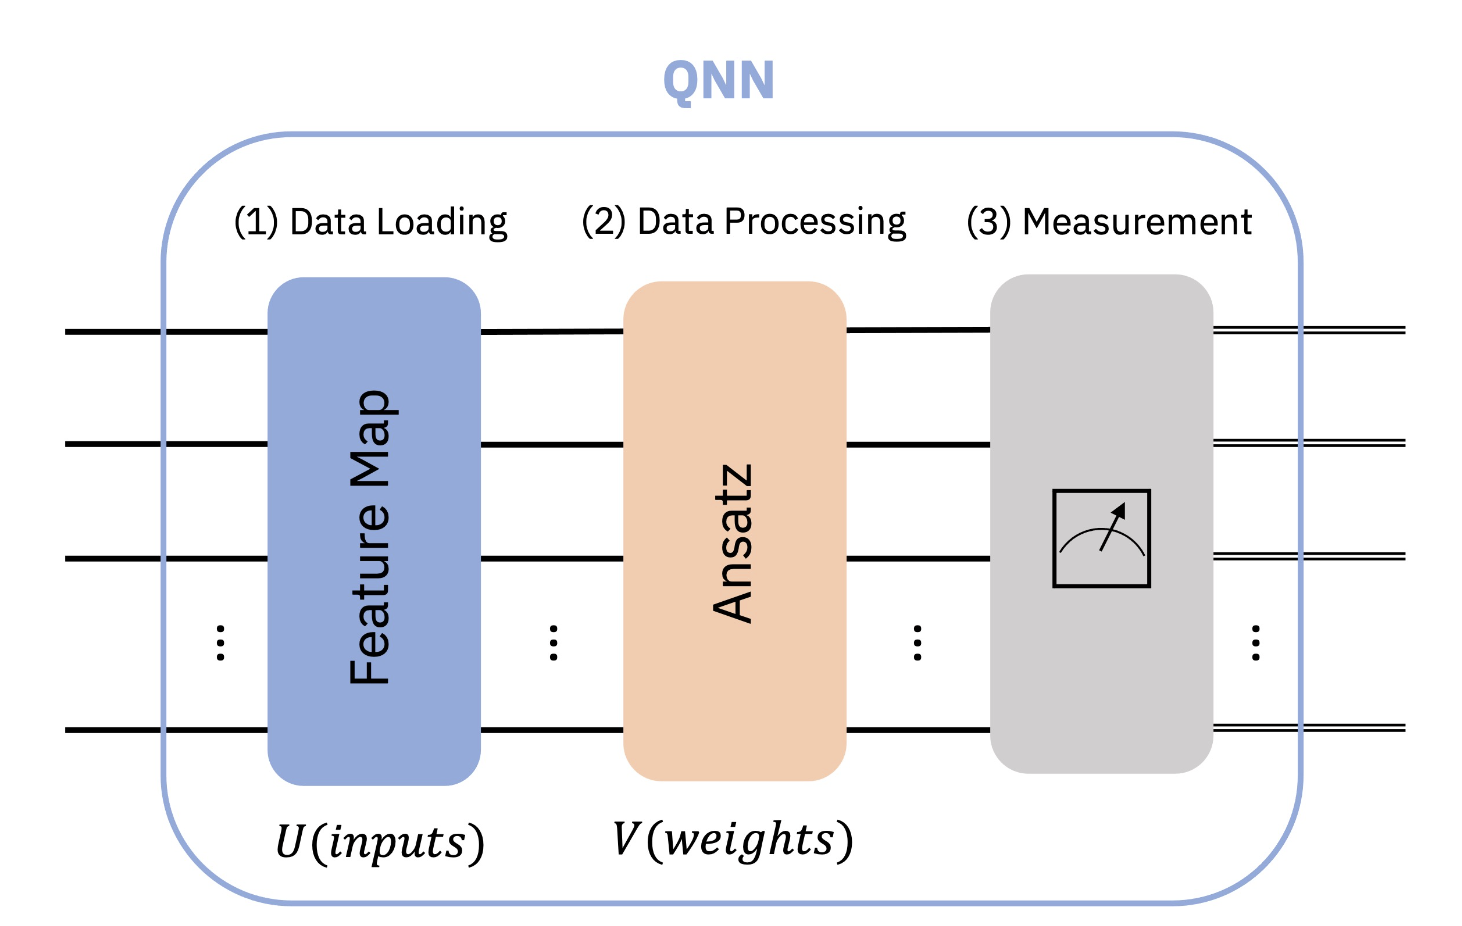
\includegraphics[width=11cm]{lib/graphics/vqc.png}
    \caption[Variational Quantum Circuit]{\ac{VQC} entnommen aus~\cite{Qiskitb}}
    \label{abb:vqc1}
\end{figure}


Ein \ac{VQC} für ein Quantum Neuronales Netzwerk besteht, wie in Abbildung~\ref{abb:vqc1} zu sehen ist aus 3 Teilen.
Die genaue Benennung der Teile variiert je nach Publikation, jedoch sind diese immer gleich aufgebaut.\footcite[Vgl.][]{McClean2018, Hu2022, Chen2022, Yu2023, Cao2023}
In dieser Arbeit wird die Bezeichnung gemäß der Darstellung in Abbildung~\ref{abb:vqc1} verwendet.
Die Feature Map ist für die Codierung der Eingabedaten verantwortlich und wird deshalb auch Data Encoding Layer genannt. Wie die Feature Map aufgebaut ist, hängt von den Eingabedaten ab.\footcite[Vgl.][S. 2]{Cao2023}
Der Ansatz, auch Variational Layer genannt, ist für die Gewichtung der Eingabedaten zuständig. Die Gewichtung wird durch die Parameter $\theta$ bestimmt.\footcite[Vgl.][S. 4]{Yu2023}
Nach der Gewichtung werden die Daten durch den Measurement Layer gemessen und als Ergebnis ausgegeben.
Das errechnete Ergebniss kann im Anschluss auf einem klassischen Computer weiter verarbeitet werden.\footcite[Vgl.][S. 9]{Chen2022}

Die Feature Map und der Variational Layer werden in den folgenden Kapiteln genauer erläutert
(siehe Kapitel~\ref{dataEncoding}~\nameref*{dataEncoding}; Kapitel~\ref{variationalLayer}~\nameref*{variationalLayer}).


\subsection{Feature Map}\label{dataEncoding}

Die Feature Map sorgt dafür, dass die klassischen Eingabedaten in Quantumzustände (beschrieben in Kapitel~\ref{qnn}) übertragen werden.\footcite[Vgl.][S. 3f.]{Yu2023}
Grunsätzlich haben Feature Maps Quantum Gates, welche als nicht trainierbare Parameter, die Eingabedaten des \ac{VQC}'s erhalten.\footcite[Vgl.][S. 2]{Hu2022}
Dadurch kommt es zu einer Veränderung der Quantumzustände und somit zu einer Veränderung der Wahrscheinlichkeiten der einzelnen Zustände.\footcite[Vgl.][S. 96]{Weigold2021}

\begin{figure}[htb]
    \centering
    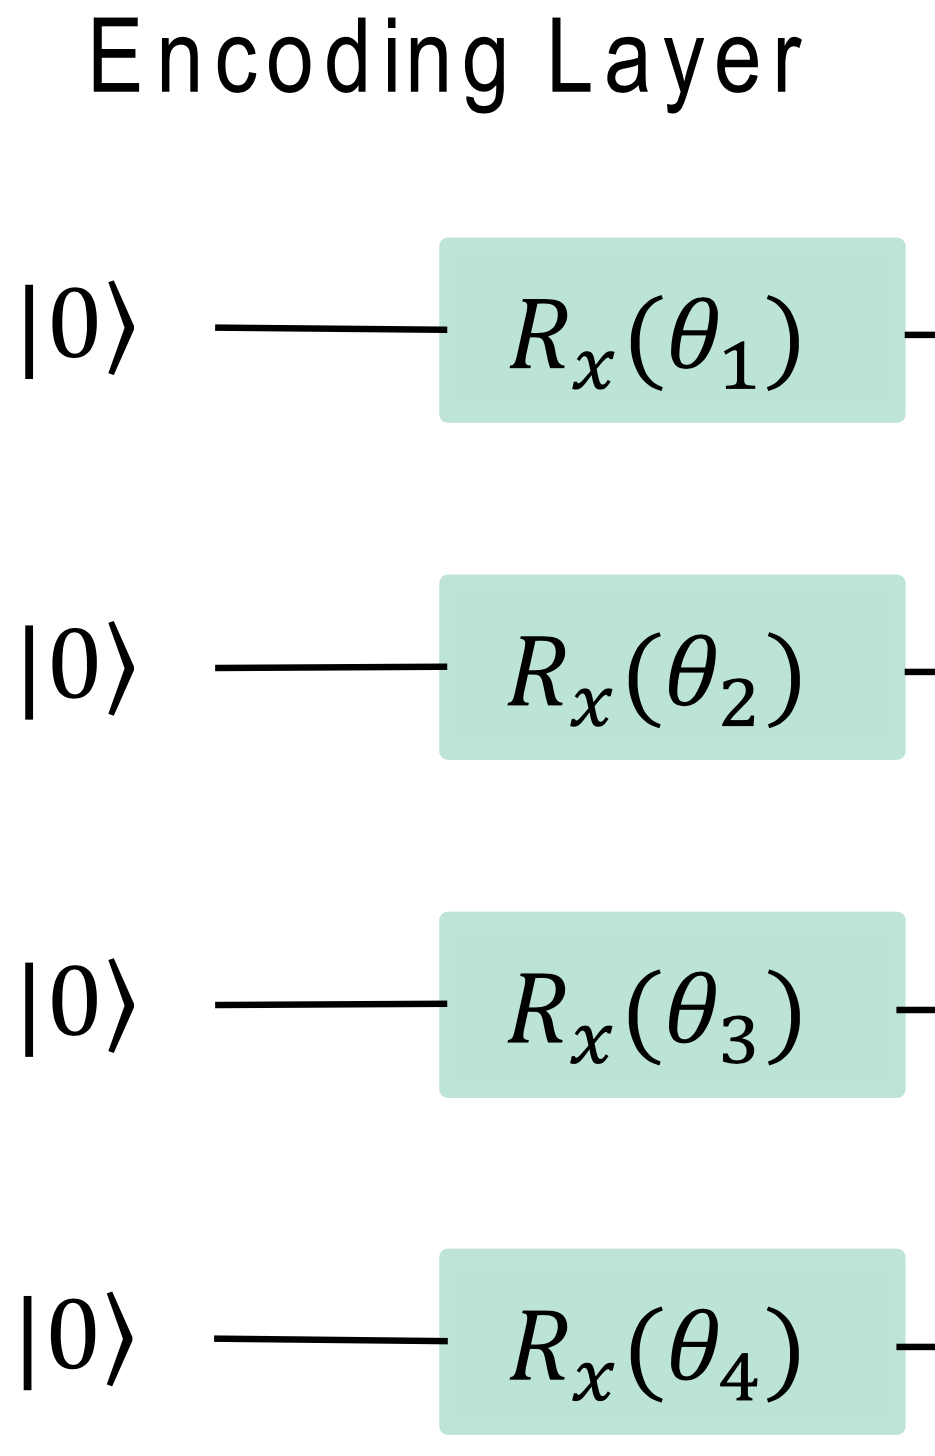
\includegraphics[width=3cm]{lib/graphics/fm_yu.png}
    \caption[Beispiel Feature Map]{Beispiel Feature Map entnommen aus~\cite[][S. 3]{Yu2023}}
    \label{abb:fm_Yu2023}
\end{figure}

In Abbildung~\ref{abb:fm_Yu2023} ist eine Feature Map zu sehen, welche die Eingabedaten $x_1, x_2$ ... $x_4$, durch eine einzelne Pauli-Rotation in einen Quantum Zustand überträgt. Solch ein Pauli-Rotation kann nur eine einfache Sinuskurve lernen, während wiederholte Pauli-Codierungen das Abbildungssprektrum linear erweitern.\footcite[Vgl.][S. 2]{Schuld2021}
Pauli-Rotationen sind die Art von Gates, welche um die \code{x}, \code{y} oder \code{z}-Achse rotieren.\footcite[Vgl.][S. 81]{Williams1998}

Welche Gates in einer Feature Maps verwendet werden, hängt von den Eingabedaten ab.\footcite[Vgl.][S. 9]{Weigold2022}
Es gibt verschiedene Arten des Encodings: Basis, Amplitude, QuAM und Angle, welche verschiedene Ergebnisse liefern.\footcite[Vgl.][S. 8]{Weigold2022}
Die später betrachteten \ac{QLSTM}-Architekturen verwenden haupsächlich das Angle Encoding.\footcite[Vgl.][]{Chen2022,Yu2023,Cao2023}
Aufgrund der Einfachheit ist diese Art des Encodings am meisten verbreitet.\footcite[Vgl.][S. 4]{OvalleMagallanes2023}
Auch andere relevante Publikationen über \ac{QNN}'s benutzen Angle Encoding.\footcite[Vgl.][]{Liu2021, Mari2020, Henderson2020, LaRose2020}

Angle Encoding benötig \code{n} Qubits, um \code{n} Eingabedaten zu codieren.
Die Qubits werden durch Rotationsgates in einen bestimmten Zustand gebracht, welcher durch die Eingabedaten als Parameter bestimmt wird.\footcite[Vgl.][S. 4]{OvalleMagallanes2023}




\subsection{Variational Layer (Ansatz)}\label{variationalLayer}

Sind die klassichen Daten durch die Feature Map in Quantumzustände übertragen, werden diese mit den Ansatz, auch Variational Layer genannt, weiter verarbeitet.
Dieser Layer besteht aus mehreren Quantum Gates, welche durch trainierbare Parameter, die Gewichtung der geladenenen Eingabedaten bestimmen.\footcite[Vgl.][S. 2]{Hu2022}
Aufgrund der trainierbaren Parameter,\footcite[Vgl.renote][S. 3]{Cao2023} funktioniert der Variational Layer ähnlich wie klassischen Netzwerken.\footcite[Vgl.][S. 414]{Kwak2021}
Wie in Abbildung~\ref{abb:varlayer} zu sehen, sind die verschiedenen Qubits miteinander verschaltet. Diese Verknüpfung wird mithilfe von Controlled-Not-Gates realisiert und gewährleistet die Verbindung aller Qubits, also sämtlicher Datenpunkte, miteinander.\footcite[Vgl.][S. 4]{Yu2023} 
Außerdem kommen Rotationsgates zum Einsatz, welche mit Parametern die Gewichtung der einzelnen Qubits bestimmen. 

\begin{figure}[htb]
    \centering
    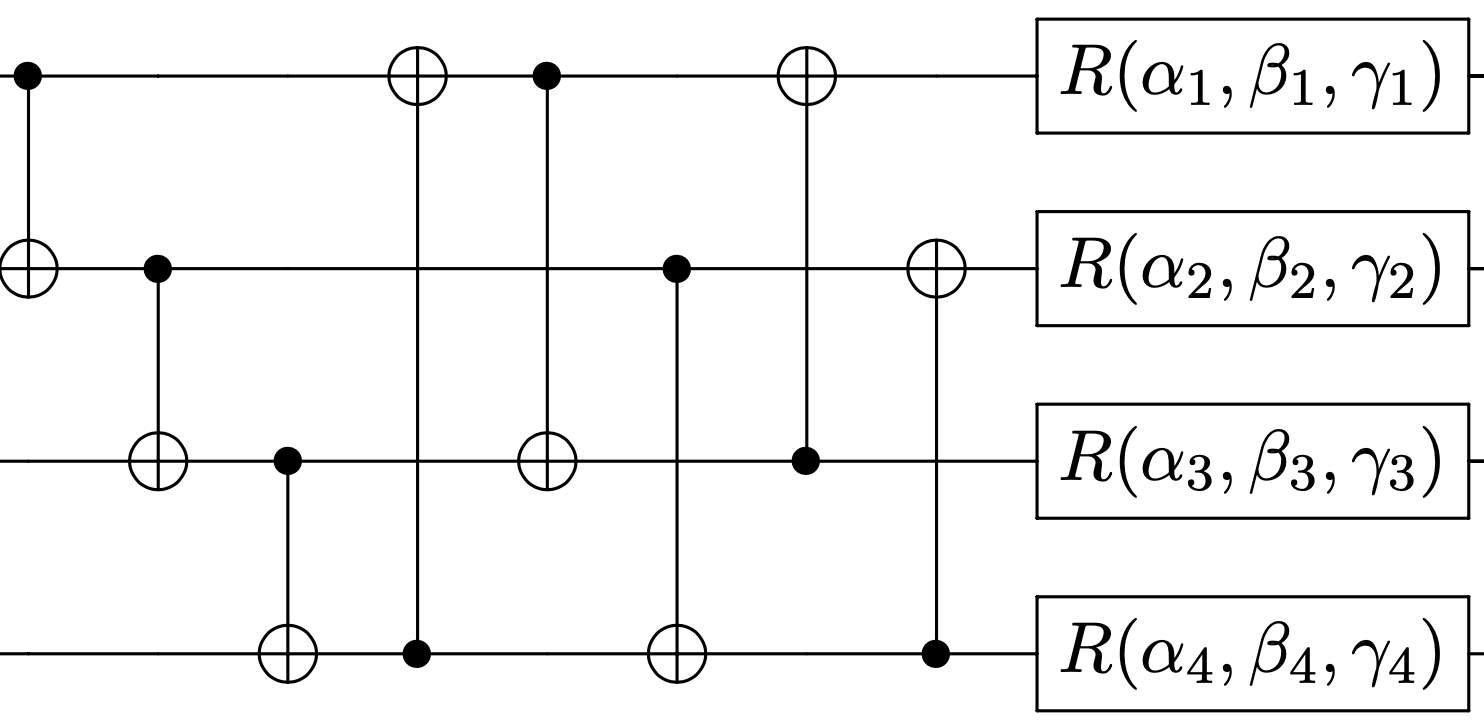
\includegraphics[width=8cm]{lib/graphics/varlayer.png}
    \caption[Beispiel Variational Layer]{Beispiel Variational Layer entnommen aus~\cite[][S. 7]{Chen2022}}
    \label{abb:varlayer}
\end{figure}

Im abbgebildeten Beispiel sind dies die trainierbaren Parameter $\alpha$, $\beta$ und $\gamma$ benannt.

Wie die Qubits miteinander verschaltet sind und welche Rotationsgates verwendet werden hängt vom Use-Case ab.\footcite[Vgl.][]{Yu2023,Chen2022,Cao2023,Sim2019}
Grundsätzlich ist es möglich Qubits und Model Komplexität hinzufügen, um die Genauigkeit des Modells zu erhöhen.\footcite[Vgl.][S. 2]{Cao2023}
Es ist möglich den Variational Layer mehrfach zu schalten, um die Tiefe des \ac{VQC}'s zu erhöhen.\footcite[Vgl.][S. 9]{Chen2022}
\cite[][S. 8]{Sim2019} diskutieren die Eignung verschiedener Circuits und untersuchen die Ausdruckswerte, beziehungsweise die Fähigkeit einen möglichst großen Datenraum abzubilden.




Welche verschiedenen Variational Layer in aktuellen Publikationen verwendet werden, wird in Kapitel~\ref{vergleichsobjekte} erläutert.


\subsection{Quantum Measurement}

Der Measurement Layer ist für die Ausgabe des \ac{VQC}'s verantwortlich, indem die Qubits gemessen und in klassiche Daten umgewandelt werden.\footcite[Vgl.][S. 2]{Cao2023}
Die Pauli matrix $\sigma_z$ (siehe Gleichung~\ref{eq:sigmaZ}) wird verwendet, um die Erwartungswerte der einzelnen Qubits zu berechnen.\footcite[Vgl.][S. 4]{Yu2023}
Nach~\cite[][]{Yu2023}, ist es möglich die Erwartungswerte der Qubits mit Frameworks zu berechnen, welche die Quantenfunktionen simulieren.

\begin{equation}
    \label{eq:sigmaZ}
    \sigma Z = \begin{bmatrix} 1 & 0 \\ 0 & -1 \end{bmatrix}
\end{equation}

\cite[][]{Busch2016} \cite[][]{Braginsky1995} und \cite[][]{Wiseman2010} setzten sich genauer mit den Thema der Quantenmessung auseinander.


\subsection{QLSTM Netzwerk Architektur}\label{qlstmArch}

Der Datenfluss bei einer \ac{QLSTM}-Zelle ist in Abbildung~\ref{abb:qlstm} dargestellt und lässt sich mathematisch durch folgende Gleichungen beschreiben:
\begin{align}
    f_t &= \sigma(VQC_1(v_t))  \\
    i_t &= \sigma(VQC_2(v_t))  \\
    \widetilde{C}_t &= \tanh(VQC_3(v_t))  \\
    c_t &= f_t \ast c_{t-1} + i_t \ast \widetilde{C}_t  \\
    o_t &= \sigma(VQC_4(v_t))  \\
    h_t &= VQC_5(o_t \ast \tanh(c_t)) \\
    y_t &= VQC_6(h_t \ast \tanh(c_t))
\end{align}
Wobei Input für $VQC_1$ bis $VQC_4$ $v_t$, die Vektor Verkettung von $x_t$ und $h_{t-1}$, ist.

\begin{figure}[htb]
    \centering
    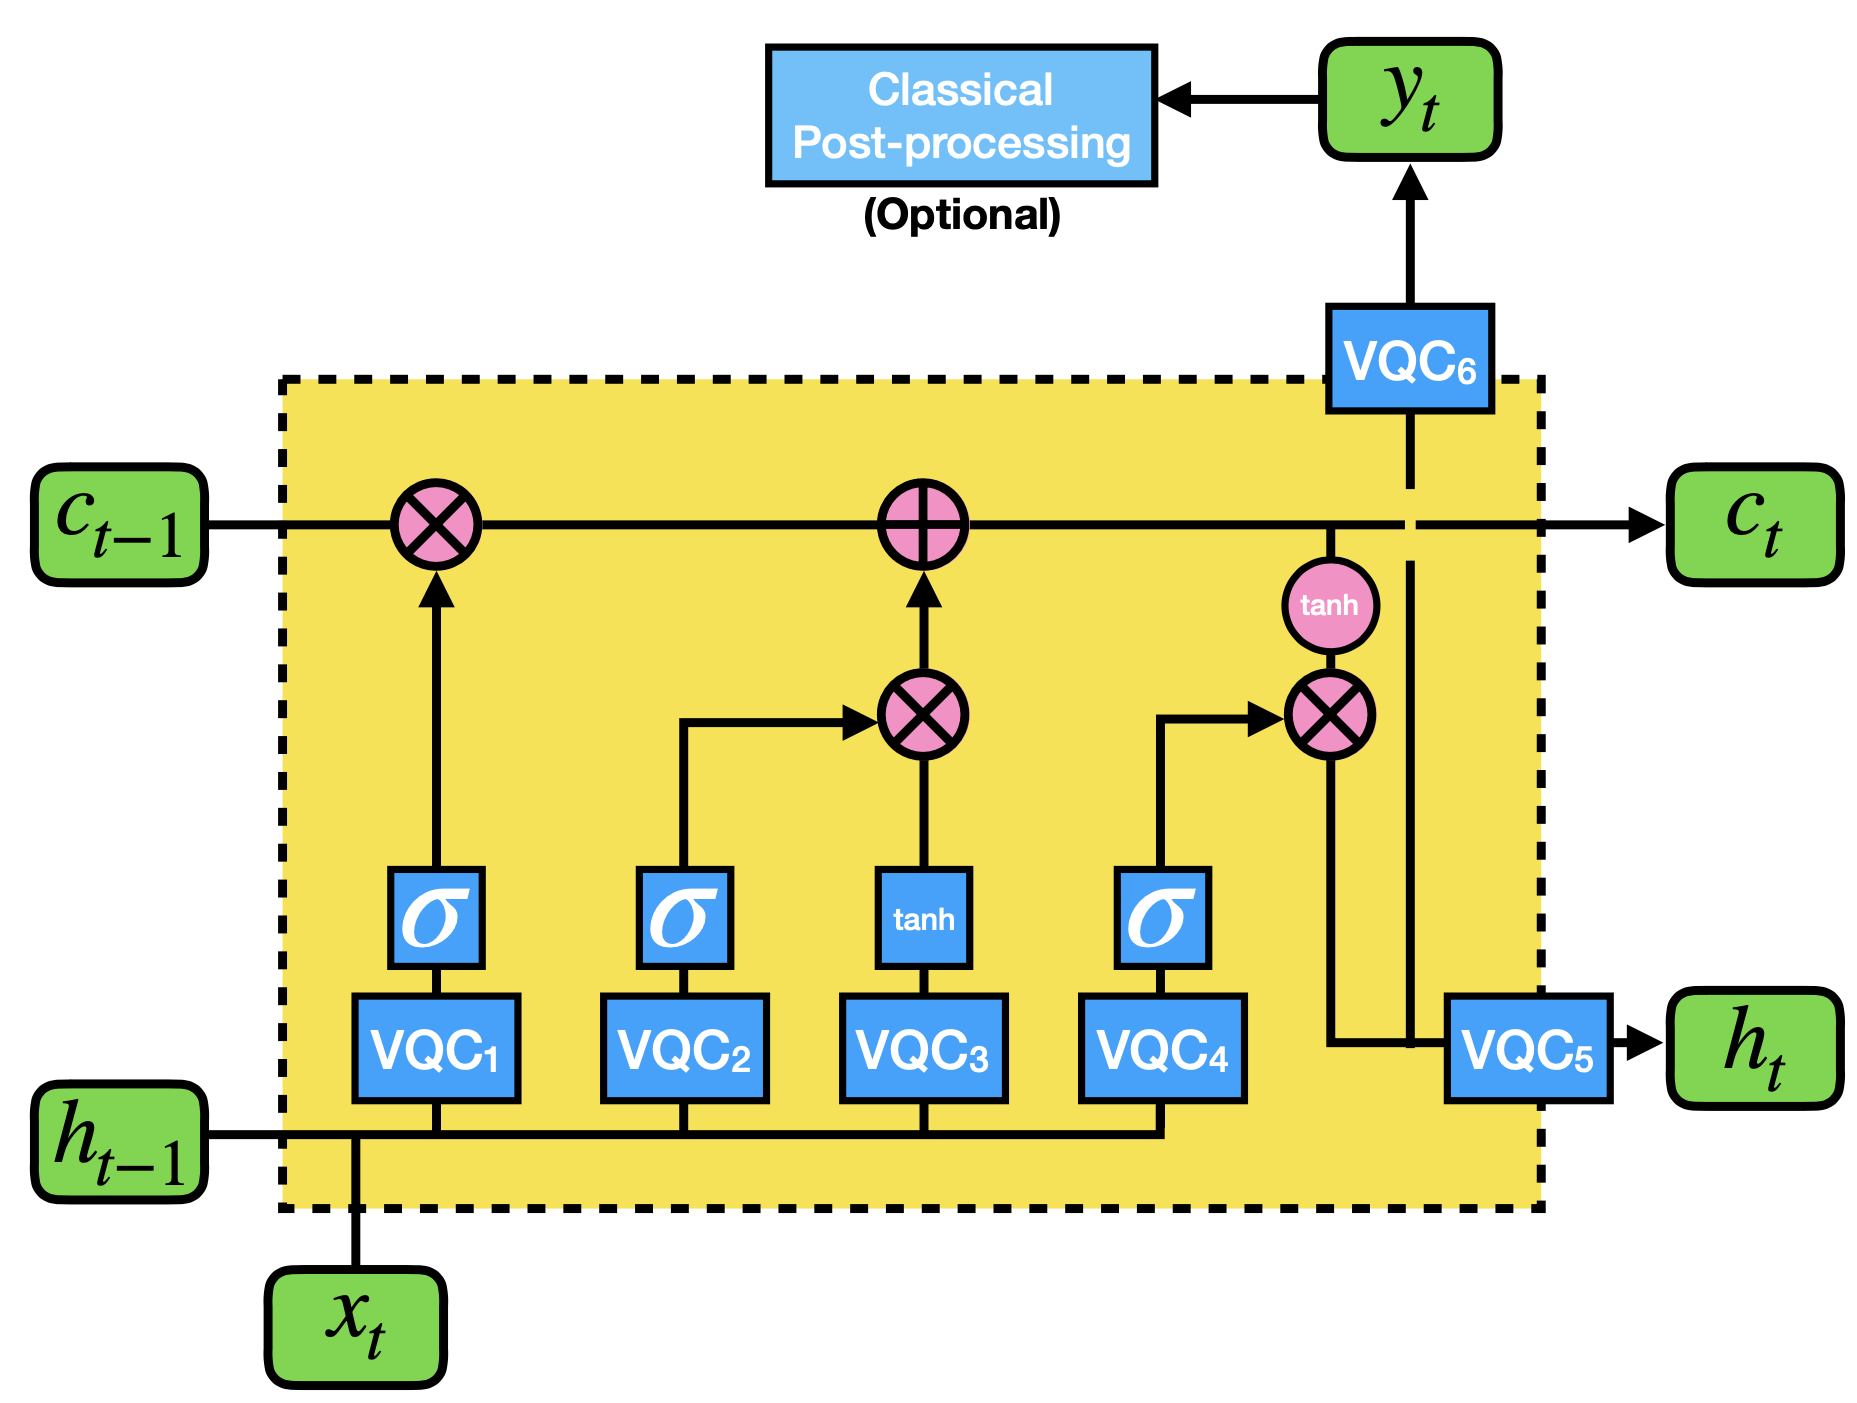
\includegraphics[width=13cm]{lib/graphics/qlstm.png}
    \caption[Quantum Long Short Term Memory Architektur]{\ac{QLSTM} Zellen Architektur entnommen aus~\cite[S. 10]{Chen2022}}
    \label{abb:qlstm}
\end{figure}

Im Vergleich zur klassichen \ac{LSTM}-Zellen Struktur, gibt es keine Gewichtsmatrizen mehr, sondern nur noch \ac{VQC}'s. Diese enthalten die trainierbaren Parameter (siehe Kapitel~\ref{variationalLayer}).
In der hier abgebildeten Architektur, gibt es sechs \ac{VQC}'s, welche die Gewichtung der Eingabedaten übernehmen. Aus diesem Grund, ist der Output $y_t$ und der Hidden State $h_t$ nicht gleich wie bei klassischen \ac{LSTM}-Architektur.
Dies hängt aber von der gewählten Anzahl der  \ac{VQC}'s ab. Während \cite[][]{Chen2022} noch sechs \ac{VQC}'s vorschlägt, schlägt~\cite[][]{Chen2023} nur noch fünf vor.
Es gibt auch Architekturen mit nur vier \ac{VQC}'s.\footcite[Vgl.][S. 4]{Yu2023}
In der Publikation von~\cite[][]{Cao2023}, werden ebenfalls 6 \ac{VQC}'s verwendet, jedoch werden diese mit klassischen Layern kombiniert.\footcite[Vgl.][S. 11]{Cao2023}
Eine Abbildung dieser Architektur ist in Anhang xy zu sehen.

Werden weniger \ac{VQC}'s verwendet, ist es möglich, dass der Output $y_t$ und der Hidden State $h_t$ gleich sind. Der sechste \ac{VQC} wird in diesem Fall nicht benötigt, da der Hidden State $h_t$ bereits die gewichteten Eingabedaten enthält.\footcite[Vgl.][S. 3]{Chen2023}
Gibt es nur vier \ac{VQC}'s, wird der Hidden State $h_t$ nicht gewichtet und der Output $y_t$ ist gleich dem Hidden State $h_t$.\footcite[Vgl.][S. 4]{Yu2023}
